\documentclass[12pt,a4paper,titlepage]{article}
\usepackage[utf8]{inputenc}
\usepackage[finnish]{babel}
\usepackage{setspace}
\usepackage{parskip}
\usepackage{amssymb}
\usepackage{amsmath}
\usepackage{graphicx}
\usepackage{fancyhdr}
\usepackage[top=1in, bottom=1in, left=1in, right=1in]{geometry}
\usepackage{float}
\usepackage[shellescape]{gmp}
\usepackage[section]{placeins}
%\usepackage[numbered,autolinebreaks,useliterate]{mcode} % jos tahdot laittaa matlabkoodia näkyville niin kannattaa käyttää tätä

% hyödyllisiä paketteja:
\usepackage{siunitx}\sisetup{per=frac} % SI-yksiköitä.
%\usepackage{supertabular} % jos tarttee isoja taulukoita
%\usepackage{fullpage} % pienemmät marginaalit jos haluaa

\usepackage{listings}
\usepackage{color}

\definecolor{dkgreen}{rgb}{0,0.6,0}
\definecolor{gray}{rgb}{0.5,0.5,0.5}
\definecolor{mauve}{rgb}{0.58,0,0.82}

\lstset{frame=tb,
  language=python,
  aboveskip=1mm,
  belowskip=1mm,
  showstringspaces=false,
  columns=flexible,
  basicstyle={\small\ttfamily},
  numbers=none,
  numberstyle=\tiny\color{gray},
  keywordstyle=\color{blue},
  commentstyle=\color{dkgreen},
  stringstyle=\color{mauve},
  breaklines=true,
  tabsize=3
}


\usepackage{hyperref} % lisääthän omat pakettisi ENNEN hyperref'iä
\hypersetup{pdfborder={0 0 0}}
\onehalfspacing
\cfoot{}
\rhead{\thepage}
% asettaa nyk. kappaleen nimen vasempaan ylänurkkaan, saa poistaa jos haluaa
\lhead{}

%%%%% kaikki ennen tätä liittyy käytettäviin paketteihin tai dokumentin muotoiluun. siihen ei tarvinne aluksi koskea. %%%%%

%%%%% kansilehti %%%%%
\title{Valkoisten kääpiöiden massa-säde relaatio}
\author{\begin{tabular}{c}
Arttu Hyvönen, 014808984
\end{tabular}}
\date{\today}
\begin{document}
\maketitle
\newgeometry{top=1in, bottom=1.5in, left=1.5in, right=1.5in}

\restoregeometry

% Sisällysluettelo
\thispagestyle{empty}
\tableofcontents
\newpage
\setcounter{page}{1}
\parskip=1em \advance\parskip by 0pt plus 2pt
\pagestyle{fancy}

% prosenttimerkillä alkavat rivit ovat kommentteja: niitä ei katsota dokumenttia käännettäessä eli ne ovat vain kirjoittajaa varten

%%%%%%%%%%%%%%% Oleellinen sisältö alkaa %%%%%%%%%%%%%%%
\section{Johdanto}

Valkoiset kääpiöt ovat tähtien, joiden massa on noin välillä $0.07\: \mathrm{M_{\odot}} -8\: \mathrm{M_{\odot}}$ ($\mathrm{M}_{\odot}$ on auringon massa), evoluution viimeinen piste. Tälle massa välille sijoittuu suuri osa galaksin tähdistä ja siksi uskotaankin, että yli 97\% tähdistä päätyy valkoisiksi kääpiöiksi (Fontaine ym. 2001). Ne syntyvät kun tähdeltä loppuu polttoaine, joka ylläpitää sen sisällä tapahtuvaa fuusiota. Ilman ytimessä tapahtuvaa fuusiota ei ole painetta, joka vastustaisi tähden oman massan aiheuttamaa painovoimaa. Silloin tähti luhistuu ja syntyy valkoinen kääpiö (Fitzpatrick 2006). 

Valkoisten kääpiöiden koko käyttäytyy melko epäintuitiivisesti. Kun niiden massa kasvaa säde ei kasva, niin kuin olettaisi, vaan pienenee. Huomataan myös, että kun lähestytään tiettyä massaa, säde näyttää lähestyvän nollaa. Toisin sanoen valkoisilla kääpiöillä on maksimi massa, jota suuremmaksi ne eivät voi kasvaa ilman, että jotain dramaattista tapahtuu (Fitzpatrick 2006).

Tässä esseessä selvitetään, mistä valkoisten kääpiöiden koon kummallinen käyttäytyminen johtuu ja mitä seurauksia sillä on. Ensin käydään läpi millä voimilla ja tähden ominaisuuksilla on vaikutusta massan ja säteen relaatioon sekä mitä oletuksia ja approksimaatioita voidaan tehdä. Sitten johdetaan relaatio ja pohditaan saatua tulosta.\\


\section{Valkoisten kääpiöiden ominaisuuksia}

Kun tähti luhistuu ja suuri määrä massaa pakkautuu pieneen tilaan, syntyy todella tiheä kappale, valkoinen kääpiö. Koska valkoiset kääpiöt ovat niin tiheitä niillä on ominaisuuksia, jotka eivät tule vastaan jokapäiväisessä elämässä. 

\subsection{Koostumus}

Valkoista kääpiötä voidaan miettiä tiheänä kaasuna, joka koostuu elektroneista ja ioneista. Tällaista kaasua kutsutaan Fermi-kaasuksi (Fitzpatrick 2006). 

Yleensä suurin osa valkoisessa kääpiössä olevista ioneista on $\mathrm{O}^{16}$ ja $\mathrm{C}^{12}$ atomien ytimiä (Straniero ym. 2003). Koska näissä ytimissä on yhtä monta protonia kuin elektronia ja tähti on kokonaisuudessaan varaukseton voidaan sanoa, että jokaista elektronia kohden ioneista tulee massa, joka vastaa kahta protonin massaa. Eli koko valkoisen kääpiön massa on $ M = 2 N m_p $, missä $N$ on elektronien lukumäärä ja $m_p$ protonin massa.

\subsection{Degeneroituminen}

Paulin kieltosääntö sanoo, että kaksi samanlaista fermionia eivät voi olla samassa kvanttitilassa. Degeneroituneeksi kaasuksi kutsutaan sellaista kaasua, jossa Paulin kieltosäännön vaikutukset alkavat olla merkittäviä, eli hiukkaset joutuvat korkeille energiatiloille muiden tilojen ollessa jo varattuja. Tätä ilmenee kun kaasu on todella tiheää, niin kuin valkoisissa kääpiöissä. (Cox ym. 2004).

Valkoisissa kääpiöissä riittää kun tarkastelee elektronien degeneroitumista koska neutronien ja protonien degeneroituminen tulee merkittäväksi vasta paljon suuremmissa tiheyksissä. Siksi tästä eteenpäin kun tarkastellaan degeneroitumista voidaan unohtaa ionien vaikutus ja puhua elektronikaasusta (Fitzpatrick 2006).

Elektronikaasulla on ominaisuus, joka on erityisen tärkeä valkoisille kääpiöille. Yleensä absoluuttisessa nollapisteessä, mikä nyt tarkoittaa, että kaasu on täysin degeneroitunutta, kaikki liike pysähtyy. Kuitenkin elektronikaasun tapauksessa elektronien liike ei pysähdy ja niillä saattaa olla suuriakin nopeuksia. Tästä johtuen kaasu aiheuttaa tarpeeksi suuren paineen, että valkoinen kääpiö ei luhistu enempää. Siis elektronikaasun degeneroituminen estää valkoisten kääpiöiden luhistumisen (Cox ym. 2004).

Todellisuudessa valkoisten kääpiöiden lämpötila ei ole lähellä absoluuttista nollapistettä. Niiden lämpötila sijoittuu välille $5000 \mathrm{K}-100000 \mathrm{K}$, mutta $T = 0$ on todettu hyväksi approksimaatioksi (Koester ym. 1990).\\


\section{Massa-säde relaatio}

Sekä ei-relativistisen että relativistisen relaation johdossa seuraillaan Fitzpatrickin (2006) luentomonistetta. 

Valkoisen kääpiön kokonaisenergia voidaan kirjoittaa muodossa
\begin{align}
E = K_{tot} + U \label{eq:e}
\end{align}
Missä $K_{tot}$ on degeneroituneiden elektronien kokonais kineettinen energia ja $U$ on hiukkasten potentiaali energia. Ionien kineettinen energia on mitätön. 

Oletetaan nyt, että tähden tiheys on vakio, jolloin potentiaali energiaksi saadaan 
\begin{align}
U = -\frac{3 G M ^2}{5 R} \label{eq:u}
\end{align}
missä $G$ on painovoima vakio, $M$ on tähden massa ja $R$ on tähden säde. Lisäksi nyt pätee luvussa 2.1 mainittu 
\begin{align}
M = 2 N m_p \label{eq:m}
\end{align}
Fermienergia on ylin energiatila, joka ei ole tyhjänä erittäin degeneroituneessa kaasussa, eli kun $T = 0$. Sitä vastaa Fermi-liikemäärä, joka on ylintä energiatilaa vastaava liikemäärä. Fermi-liikemäärä voidaan nyt kirjoittaa muodossa
\begin{align}
p_F = \hbar \left( 3 \pi^2 \frac{N}{V} \right)^{1/3} \label{eq:pf}
\end{align}
missä $N$ on elektronien lukumäärä, $\hbar$ on redusoitu Planckin vakio ja $V = \frac{3}{4} \pi R^3$. Yhtälöstä \eqref{eq:pf} voidaan nyt selvittää niiden hiukkasten lukumäärä, joiden liikemäärän suuruus on välillä $[p, p+\mathrm{d}p]$.
\begin{align}
\mathrm{d}N = \frac{V}{\pi^2 \hbar^3} p^2 \mathrm{d}p
\end{align}
Sitten integroidaan hiukkasten kineettistä energiaa kaikkien liikemäärien yli, eli välillä $[0, p_F]$ ja kerrotaan vastaavalla lukumäärällä $\mathrm{d}N$. Näin saadaan
\begin{align}
K_{tot} = \frac{V}{\pi^2 \hbar^3} \int_0^{p_F} K(p) p^2 \mathrm{d}p \label{eq:k}
\end{align}
missä $K(p)$ on yhden hiukkasen kineettinen energia liikemäärän avulla lausuttuna.


\subsection{Ei-relativistinen}
Tarkastellaan ensin ei-relativistista tapausta, joka pätee kun $M \ll M_{\odot}$. Nyt $K(p)$ on klassinen kineettinen energia eli $K(p) = p^2/2 m$. Sijoitetaan $K(p)$ yhtälöön \eqref{eq:k}, jolloin saadaan
\begin{align}
K_{tot} = \frac{V}{\pi^2 \hbar^3} \int_0^{p_F} \left(\frac{p^2}{2 m}\right) p^2 \mathrm{d}p 
\end{align}
missä $m = m_e$, joka on elektronin massa. Tästä yhtälöstä saadaan integroinnin ja sievennyksen jälkeen muoto kokonais kineettiselle energialle. Kun tähän vielä sijoitetaan yhtälö \eqref{eq:m} ja tilavuudelle muoto säteen avulla, saadaan
\begin{align}
K_{tot} = \frac{3 \hbar^2}{20 m_e} \left( \frac{9}{8} \pi \right)^{2/3} \left(\frac{M}{m_p} \right)^{5/3} \frac{1}{R^2}
\end{align}
Sitten jos vielä sijoitetaan tämä yhtälön \eqref{eq:u} kanssa yhtälöön \eqref{eq:e} saadaan kokonais energialle muoto
\begin{align}
E = \frac{A}{R^2} - \frac{B}{R} 
\end{align}
missä $A \propto M^{5/3}$ ja $B \propto M^2$. Nyt haettu säde on energian minimissä, jonka voi löytää helposti etsimällä derivaatan $\frac{\mathrm{d}E}{\mathrm{d}R}$ nollakohdat. Saadaan relaatio
\begin{align}
R = \frac{2 A}{B} \propto M^{-1/3} \label{eq:eirela}
\end{align}

\subsection{Erittäin relativistinen}
Relativistisessa tapauksessa $K(p) = \sqrt{p^2 c^2 + m_e^2 c^4}$, johon on tullut mukaan elektronien sisäenergia. Nyt erittäin relativistinen tapaus tarkoittaa sitä, että $p \gg m_ec$ jolloin voidaan approksimoida
\begin{align}
K(p) = p^3 c + \frac{m_e^2 c^3}{2} p + ...
\end{align} 
Lisäksi erittäin relativistinen tapaus tarkoittaa myös sitä, että se pätee vain kun massa on suuri. Sijoitetaan ensimmäiset termit yhtälöön \eqref{eq:k}, jolloin saadaan
\begin{align}
K_{tot} = \frac{V}{\pi^2 \hbar^3} \int_0^{p_F} \left( p^3 c + \frac{m_e^2 c^3}{2} p \right) p^2 \mathrm{d}p
\end{align}
Integroinnin ja sijoituksien jälkeen kokonais energialle saadaan muoto
\begin{align}
E = \frac{A-B}{R}+C R 
\end{align}
missä $A \propto M^{4/3}$, $B \propto M^{2}$ ja $C \propto M^{2/3}$. Nyt massa-säde relaatio voidaan selvittää etsimällä energian minimi. Saadaan
\begin{align}
R = \sqrt{\frac{A-B}{C}} \propto \sqrt{M^{2/3}-M^{4/3}} \label{eq:rela}
\end{align}
Tästä huomataan heti, että $R$ saa reaalisia arvoja vain silloin kun $A > B$ ja kun $A = B$ seuraa $R = 0$. Eli on olemassa raja massalle, jonka jälkeen valkoinen kääpiö luhistuu elektronikaasun paineesta huolimatta. Tätä rajaa kutsutaan Chandrasekharin rajaksi. 

\subsection{Yleisempi relaatio}

Kuvassa \ref{pic:1} on piirretty lukujen 3.1 ja 3.2 relaatiot sekä merkitty relativistisessa tapauksessa ilmennyt raja massalle, joka tehdyillä oletuksilla saa arvon $1.72 \mathrm{M}_{\odot}$.
\begin{figure}[H]
\centering
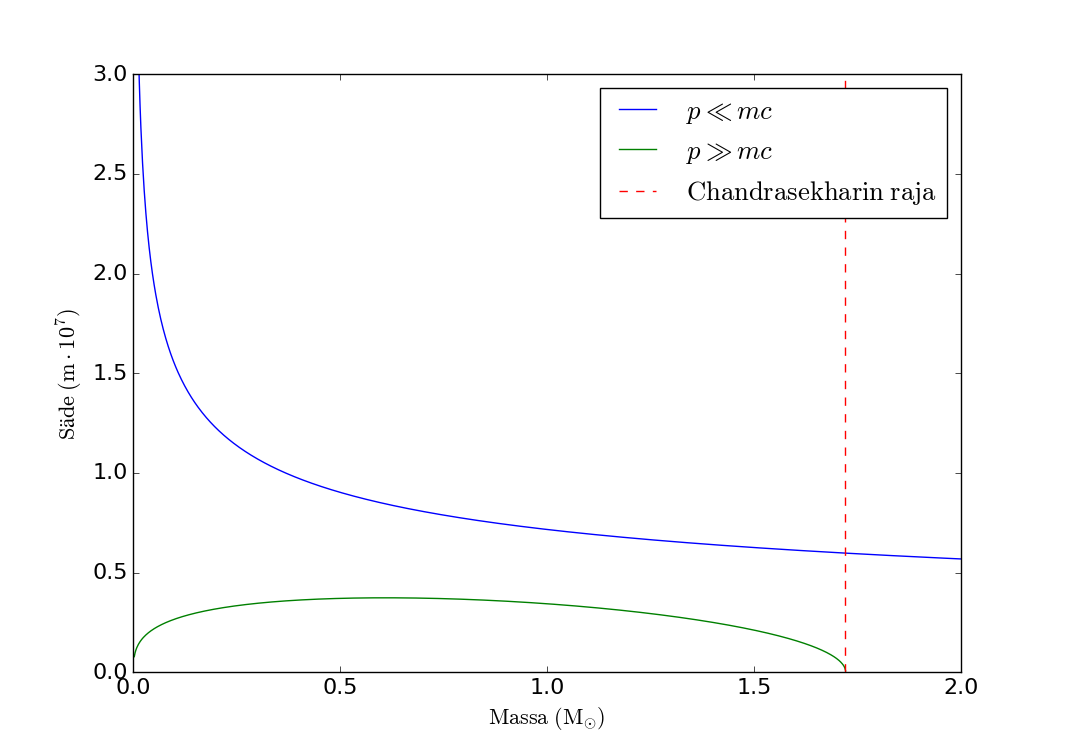
\includegraphics[width=\textwidth]{mr1.png}
\caption{Ei-relativistinen ja erittäin relativistinen relaatio}
\label{pic:1}
\end{figure}
Kuvasta \ref{pic:1} huomaa myös selvästi, kuinka nyt saadut relaatiot ovat vajavaisia, eivätkä ne pysty edes yhdessä kuvaamaan massa-säde relaatiota muualla kuin ääritapauksissa. Erityisesti tiheyden olettaminen vakioksi on melko huono approksimaatio, vaikkakin tulokset ovat oikeaa kokoluokkaa.
\newpage
Valkoisille kääpiöille on johdettu tarkempia massa-säde relaatioita, joissa ei oleteta tähden tiheyttä vakioksi. Tällaisen relaation johtoon voi lähteä esimerkiksi yleisesti tähdille pätevillä yhtälöillä
\begin{align}
\frac{\mathrm{d}p}{\mathrm{d}r} &= - \frac{G \rho(r) m(r)}{r^2} \\
\frac{\mathrm{d}m}{\mathrm{d}r} &= \rho(r) 4 \pi r^2
\end{align}
joissa $\rho(r)$ on tiheyden funktio, $m(r)$ on massa säteen $r$ sisäpuolella ja $p$ on paine (Sagert ym. 2005). Lisäksi voidaan relaatiossa ottaa huomioon myös yleisen suhteellisuusteorian vaikutukset käyttämällä edellisten yhtälöiden sijasta Tolman-Oppenheimer-Volkoff (TOV) yhtälöitä (Carvalho ym. 2015). Kuvassa \ref{pic:2} on sovitus massa-säde relaatiolle TOV yhtälöiden avulla, käyttäen samaa muotoa kuin Carvalho ym. (2015) ja vertailun vuoksi mukana luvussa 3.1 johdettu muoto.
\begin{figure}[H]
\centering
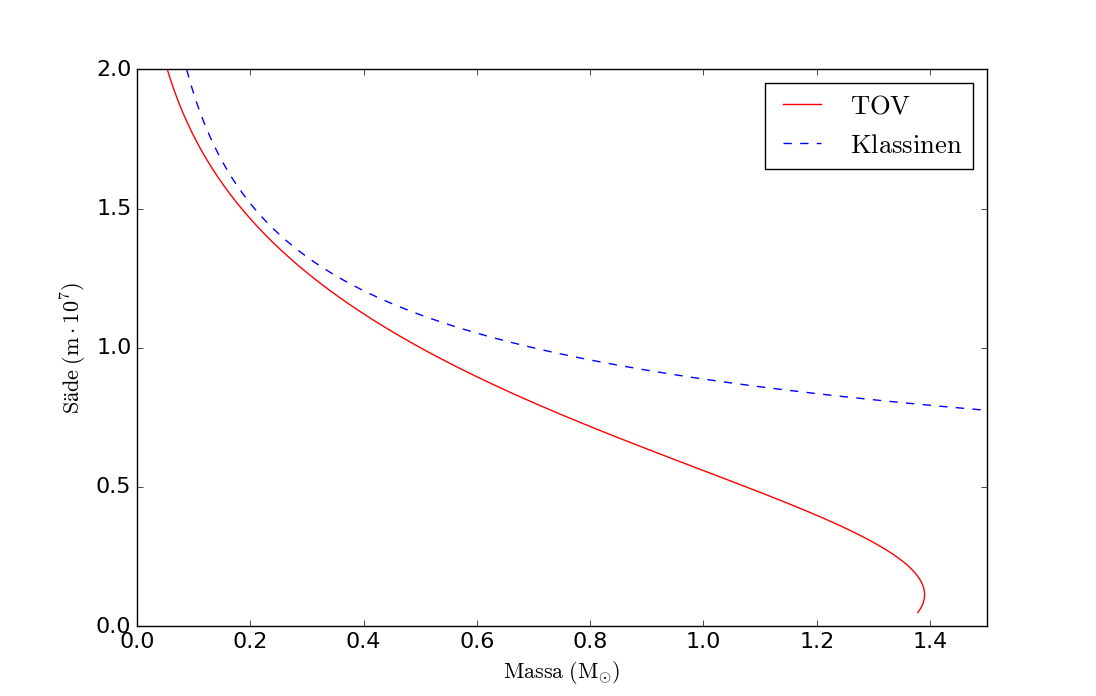
\includegraphics[width=\textwidth]{mr2.png}
\caption{Massa-säde relaatio TOV yhtälöitä käyttämällä}
\label{pic:2}
\end{figure}

\subsection{Chandrasekharin raja}
Luvussa 3.2 huomattiin, että valkoiset kääpiöt eivät voi olla tiettyä massaa suurempia. Silloin rajalle saatiin arvoksi $1.72 \mathrm{M}_{\odot}$. Nykyään hyväksytty arvo rajalle on noin $1.4 \mathrm{M}_{\odot}$ riippuen tähden koostumuksesta (Carvalho ym. 2015, Fitzpatrick 2006). 

Tietenkin herää kysymys, mitä tapahtuu jos valkoiseen kääpiöön lisätään massaa tämän rajan jälkeen. Kuten luvussa 3.2 mainittiin, tämän rajan jälkeen elektronikaasun aiheuttama paine ei ole tarpeeksi suuri, jotta se pystyisi vastustamaan gravitaatiota, minkä vuoksi valkoinen kääpiö alkaa luhistua. Tämän luhistumisen myötä elektronit ja protonit alkavat yhdistyä, muodostaen neutroneita. Näin tähdestä tulee laskennallisesti elektronikaasun sijasta neutronikaasua. Tämä neutronikaasu jatkaa luhistumistaan niin kauan, että siitä tulee degeneroitunutta ja tästä aiheutuva paine pysäyttää luhistumisen. Tällaista tähteä kutsutaan neutronitähdeksi (Fitzpatrick 2006).

Jos valkoiseen kääpiöön todellisuudessa lisätään massaa niin kauan, että se lähestyy Chandrasekharin rajaa se ei välttämättä luhistu neutronitähdeksi. On tehty havaintoja kaksoistähti systeemeistä, joissa toinen tähti on valkoinen kääpiö, joka saa pikkuhiljaa massaa toiselta tähdeltä. Kun tämä valkoinen kääpiö lähestyy Chandrasekharin rajaa korkea lämpötila aiheuttaa ydinreaktion, jonka seurauksen valkoinen kääpiö räjähtää jättämättä jäännöstä. Tätä räjähdystä kutsutaan tyypin Ia supernovaksi (Mazzali ym. 2007). \\

\section{Johtopäätökset}

Kuten pääsarjan tähdillä myös valkoisilla kääpiöillä kahden voiman, sisäisen paineen ja gravitaation, tasapaino on elinehto. Pääsarjan tähdillä paineen luo ytimessä tapahtuvat ydinreaktiot ja valkoisilla kääpiöillä samassa roolissa on Paulin kieltosäännöstä seuraava elektronien degeneraation aiheuttama paine.

Valkoisilla kääpiöillä tasapainon säilymiseksi täytyy säteen pienentyä massan kasvaessa. Massan ja säteen relaation voi laskea usealla tavalla riippuen siitä, mitä haluaa ottaa huomioon. Kuitenkin kaikki tulokset, jotka pätevät suuremmille massoille, näyttävät, että on olemassa Chandrasekharin raja, jonka jälkeen ei tasapaino ole enää mahdollinen. Valkoista kääpiötä massiivisemmat tiheät kappaleet ovat neutronitähtiä, mutta yleensä jos luonnossa valkoinen kääpiö saa lisää massaa ajan kuluessa se räjähtää supernovana.


\newpage
\section{Lähdeluettelo}
{\footnotesize 
G. Fontaine, P. Brassard \& P. Bergeron 2001. The Potential of White Dwarf Cosmochronology. Astronomical Society of the Pacific 113, 409–435.
 
R. Fitzpatrick 2006. Thermodyamics and Statistical Mechanics. The University of Texas at Austin.

O. Straniero, I. Domínguez, G. Imbriani \& L. Piersanti 2003. The Chemical Composition of White Dwarfs as a Test of Convective Efficiency during Core Helium Burning. The Astrophysical Journal 583, 878–884.

J. P. Cox \& R. T. Giuli 2004. Cox \& Giuli's principles of stellar structure. Cambridge Scientific Publishers. 

D. Koester \& G. Chanmugam 1990. Physics of white dwarf stars. Reports on Progress in Physics 53, 837-915.

I. Sagert, M Hempel, C. Greiner \& J. Schaffner–Bielich 2006. Compact Stars for Undergraduates. European Journal of Physics 27, 577-610.

G. A. Carvalho, R. M. Marinho Jr \& M. Malheiro 2015. Mass-Radius diagram for compact stars. Journal of Physics: Conference Series 630.

P. A. Mazzali, F. K. Röpke, S. Benetti \& W. Hillebrandt 2007. A Common Explosion Mechanism for Type Ia Supernovae. Science 315, 825-828.
}


%%%%% Sisältö loppuu, lähdeluettelo %%%%%
\bibliographystyle{plain}
\bibliography{selkkarilahteet} %lähdeluettelon tiedot tiedostossa selkkarilahteet.bib. Esimerkiksi helkasta saa kirjojen tiedot valmiiksi bibtex-muodossa, kannattaa hyödyntää.

\appendix

\end{document}